\chapter{Cibles de fonctionnement}

\section{Les attentes client}

	Les clients ont certaines attentes lorsqu'ils signent un contrat (qui varient selon le client). Ci dessous nous allons lister les plus importantes d'entre elles qui peuvent apparaitre.

\begin{itemize}
	\item une certaine proximité (couvrir le territoire)~;
	\item un support technologique~;
	\item de l'innovation~;
	\item de l'expertise~;

	\item assurer la gestion contractuelle et le reporting~;
	\item gérer les interventions (intervention forfaitaire : préventive et curative standard ; intervention en bon de commande : curative exceptionnelle, amélioration installations, traitement obsolescence...)~;
	\item une identification des risques techniques, financiers et organisationnels~;
	\item un compte rendu de l'état des lieux initial (pour les soldes d'écart si des travaux en plus sont nécessaires~;

	\item une améliorer le cadre de vie~;
	\item un respecter l'environnement~;

	\item un accompagnement dans la conception, la réalisation, l'exploitation et la maintenance~; d'installations plus économes en énergie et plus respectueuse de l'environnement~;
	\item un suivi des spécifications du client~;
	\item un suivi des avancements pour le client~;
	\item une construction et validation des processus avec le client~;
	\item une revue périodique du contrat pour les décisions à renouveler ou non, et la prise en compte de réclamations du client~;
	\item des preuves du respect des engagements (bonne mise en oeuvre, et adaptation au besoin).
\end{itemize}


\section{Les nouvelles règles de gestion}
Dans cette partie, nous allons proposer certaines règles standard qui pourront aider à réduire les dysfonctionnements dans la gestion des contrats de maintenance.



\section{Processus Retour d'exéprience}

\begin{figure}[h!]
	\centering
	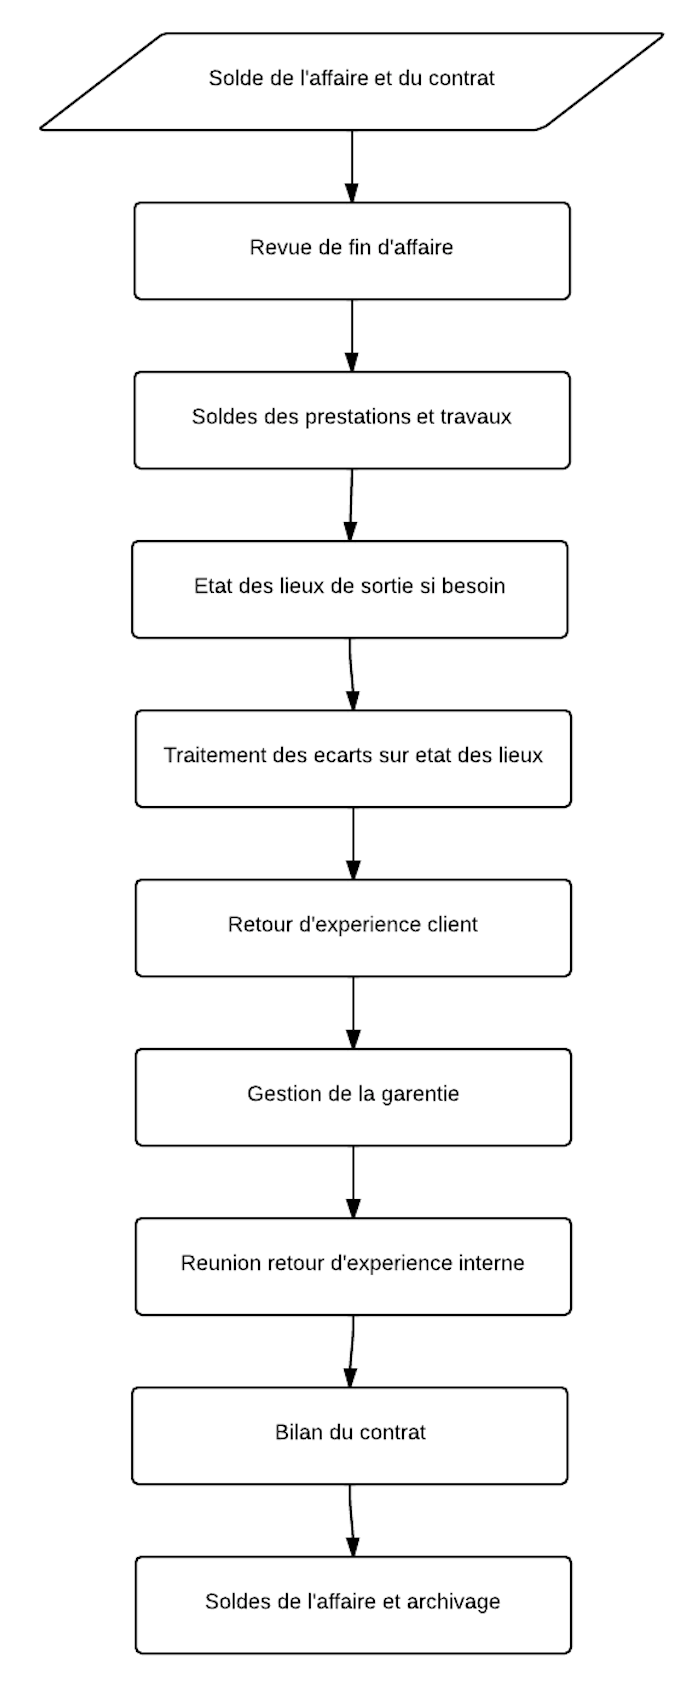
\includegraphics[width=0.45\linewidth]{images/processus_retour_experience.png}
	\caption{Processus de retour d'experience}
	\label{fig:processusRetourExperience}
\end{figure}

Ainsi l'ajout du processus \textit{retour d'\'exp\'erience client} dans le sous-processus \textit{solde
de l'affaire et du contrat} r\'epond aux exigences de SPIE Sud Est suivante~:

\begin{itemize}
    \item Base de connaissance m\'etier type de contrat~;
    \item Identification des risques techniques/financiers/organisationnels.
\end{itemize}


